\documentclass[11pt,compress,t,notes=noshow, xcolor=table]{beamer}
\usepackage[]{graphicx}\usepackage[]{color}
% maxwidth is the original width if it is less than linewidth
% otherwise use linewidth (to make sure the graphics do not exceed the margin)
\makeatletter
\def\maxwidth{ %
  \ifdim\Gin@nat@width>\linewidth
    \linewidth
  \else
    \Gin@nat@width
  \fi
}
\makeatother

\newcommand{\citebutton}[2]{%
\beamergotobutton{\href{#2}{#1}}%
}

\newcommand{\blu}[1]{\textcolor{blue}{#1}}
\newcommand{\org}[1]{\textcolor{orange}{#1}}
\newcommand{\ques}{\textbf{\textcolor{red}{Question:  }}}
\newcommand{\questionssofar}{\begin{frame}\frametitle{Any questions?}\end{frame}}

\newcommand\warning{%
 \makebox[1.4em][c]{%
 \makebox[0pt][c]{\raisebox{.1em}{\scriptsize!}}%
 \makebox[0pt][c]{\color{red}\normalsize$\bigtriangleup$}}}%

\definecolor{fgcolor}{rgb}{0.345, 0.345, 0.345}
\newcommand{\hlnum}[1]{\textcolor[rgb]{0.686,0.059,0.569}{#1}}%
\newcommand{\hlstr}[1]{\textcolor[rgb]{0.192,0.494,0.8}{#1}}%
\newcommand{\hlcom}[1]{\textcolor[rgb]{0.678,0.584,0.686}{\textit{#1}}}%
\newcommand{\hlopt}[1]{\textcolor[rgb]{0,0,0}{#1}}%
\newcommand{\hlstd}[1]{\textcolor[rgb]{0.345,0.345,0.345}{#1}}%
\newcommand{\hlkwa}[1]{\textcolor[rgb]{0.161,0.373,0.58}{\textbf{#1}}}%
\newcommand{\hlkwb}[1]{\textcolor[rgb]{0.69,0.353,0.396}{#1}}%
\newcommand{\hlkwc}[1]{\textcolor[rgb]{0.333,0.667,0.333}{#1}}%
\newcommand{\hlkwd}[1]{\textcolor[rgb]{0.737,0.353,0.396}{\textbf{#1}}}%
\let\hlipl\hlkwb

\usepackage{framed}
\makeatletter
\newenvironment{kframe}{%
 \def\at@end@of@kframe{}%
 \ifinner\ifhmode%
  \def\at@end@of@kframe{\end{minipage}}%
  \begin{minipage}{\columnwidth}%
 \fi\fi%
 \def\FrameCommand##1{\hskip\@totalleftmargin \hskip-\fboxsep
 \colorbox{shadecolor}{##1}\hskip-\fboxsep
     % There is no \\@totalrightmargin, so:
     \hskip-\linewidth \hskip-\@totalleftmargin \hskip\columnwidth}%
 \MakeFramed {\advance\hsize-\width
   \@totalleftmargin\z@ \linewidth\hsize
   \@setminipage}}%
 {\par\unskip\endMakeFramed%
 \at@end@of@kframe}
\makeatother

\definecolor{shadecolor}{rgb}{.97, .97, .97}
\definecolor{messagecolor}{rgb}{0, 0, 0}
\definecolor{warningcolor}{rgb}{1, 0, 1}
\definecolor{errorcolor}{rgb}{1, 0, 0}
\newenvironment{knitrout}{}{} % an empty environment to be redefined in TeX

\usepackage{alltt}
\newcommand{\SweaveOpts}[1]{}  % do not interfere with LaTeX
\newcommand{\SweaveInput}[1]{} % because they are not real TeX commands
\newcommand{\Sexpr}[1]{}       % will only be parsed by R
\newcommand{\xmark}{\ding{55}}%


\usepackage[english]{babel}
\usepackage[utf8]{inputenc}

\usepackage{dsfont}
\usepackage{verbatim}
\usepackage{amsmath}
\usepackage{amsfonts}
\usepackage{amssymb}
\usepackage{bm}
\usepackage{csquotes}
\usepackage{multirow}
\usepackage{longtable}
\usepackage{booktabs}
\usepackage{enumerate}
\usepackage[absolute,overlay]{textpos}
\usepackage{psfrag}
\usepackage{algorithm}
\usepackage{algpseudocode}
\usepackage{eqnarray}
\usepackage{arydshln}
\usepackage{tabularx}
\usepackage{placeins}
\usepackage{tikz}
\usepackage{setspace}
\usepackage{colortbl}
\usepackage{mathtools}
\usepackage{wrapfig}
\usepackage{bm}
\usepackage{amsmath}
\usepackage{pifont}

\usetikzlibrary{shapes.multipart,shapes,arrows,automata,positioning,calc,chains,trees, shadows}
\tikzset{
  %Define standard arrow tip
  >=stealth',
  %Define style for boxes
  punkt/.style={
    rectangle,
    rounded corners,
    draw=black, very thick,
    text width=6.5em,
    minimum height=2em,
    text centered},
  % Define arrow style
  pil/.style={
    ->,
    thick,
    shorten <=2pt,
    shorten >=2pt,}
}

\tikzstyle{vec}=[draw, rectangle, fill = white, minimum width=5mm, minimum height=1cm, inner sep = 2pt]

\usepackage{subfig}

% Defines macros and environments
\usepackage{../../style/lmu-lecture}


\let\code=\texttt
\let\proglang=\textsf

\setkeys{Gin}{width=0.9\textwidth}

\setbeamertemplate{frametitle}{\expandafter\uppercase\expandafter\insertframetitle}

\usepackage{bbm}
% basic latex stuff
\newcommand{\pkg}[1]{{\fontseries{b}\selectfont #1}} %fontstyle for R packages
\newcommand{\lz}{\vspace{0.5cm}} %vertical space
\newcommand{\dlz}{\vspace{1cm}} %double vertical space
\newcommand{\oneliner}[1] % Oneliner for important statements
{\begin{block}{}\begin{center}\begin{Large}#1\end{Large}\end{center}\end{block}}


%new environments
\newenvironment{vbframe}  %frame with breaks and verbatim
{
 \begin{frame}[containsverbatim,allowframebreaks]
}
{
\end{frame}
}

\newenvironment{vframe}  %frame with verbatim without breaks (to avoid numbering one slided frames)
{
 \begin{frame}[containsverbatim]
}
{
\end{frame}
}

\newenvironment{blocki}[1]   % itemize block
{
 \begin{block}{#1}\begin{itemize}
}
{
\end{itemize}\end{block}
}

\newenvironment{fragileframe}[2]{  %fragile frame with framebreaks
\begin{frame}[allowframebreaks, fragile, environment = fragileframe]
\frametitle{#1}
#2}
{\end{frame}}


\newcommand{\myframe}[2]{  %short for frame with framebreaks
\begin{frame}[allowframebreaks]
\frametitle{#1}
#2
\end{frame}}

\newcommand{\remark}[1]{
  \textbf{Remark:} #1
}


\newenvironment{deleteframe}
{
\begingroup
\usebackgroundtemplate{
\includegraphics[width=\paperwidth,height=\paperheight]{../style/color/red.png}}
 \begin{frame}
}
{
\end{frame}
\endgroup
}
\newenvironment{simplifyframe}
{
\begingroup
\usebackgroundtemplate{
\includegraphics[width=\paperwidth,height=\paperheight]{../style/color/yellow.png}}
 \begin{frame}
}
{
\end{frame}
\endgroup
}\newenvironment{draftframe}
{
\begingroup
\usebackgroundtemplate{
\includegraphics[width=\paperwidth,height=\paperheight]{../style/color/green.jpg}}
 \begin{frame}
}
{
\end{frame}
\endgroup
}
% https://tex.stackexchange.com/a/261480: textcolor that works in mathmode
\makeatletter
\renewcommand*{\@textcolor}[3]{%
  \protect\leavevmode
  \begingroup
    \color#1{#2}#3%
  \endgroup
}
\makeatother





\input{../../latex-math/basic-math.tex}
\input{../../latex-math/basic-ml.tex}

%\newcommand{\titlefigure}{figure/gpt_sq.png}
\newcommand{\learninggoals}{
\item Learn about different techniques to reduce compute and memory
\item Learn about distributed training with data/tensor parallelism
\item Learn about FlashAttention
}
\definecolor{texblue}{rgb}{0, 0, 1}
\def\myblue#1{\textcolor{texblue}{#1}}

\title{Training Large Language Models}
% \author{}
\institute{\href{https://slds-lmu.github.io/lecture_dl4nlp/}{slds-lmu.github.io/lecture\_dl4nlp}}
\date{}

\begin{document}
\lecturechapter{How to reduce memory and compute}
\lecture{Deep Learning for NLP}


%Notes:
% Slides: https://jasonwei20.github.io/files/FLAN%20talk%20external.pdf
% Check out emergence talk: https://www.youtube.com/watch?v=0SuyDLjNR9g

% LLM Survey: https://arxiv.org/pdf/2303.18223.pdf

% ------------------------------------------------------------------------------

\begin{vbframe}{Distributed Training}

\vfill

\begin{itemize}
 	\item Training LLMs faster on many GPUs
 	\item Avoiding OOM issues
	\item \textbf{Data parallelism:} split the data on different model replicas
	\item \textbf{Tensor parallellism:} split model parameters accross GPUs
% 	\item \textbf{Sharded optimizers:} reduce optimizer overhead by No. GPUs
% 	\begin{itemize}
% 	 	\item ZeRO (Zero Redundancy Optimizer)
% 		\item Requires low extra communication between GPUs
% 	 	\item Decreases optimizer memory requirement
% 		\item Improves training speed
% \end{itemize}
\end{itemize}

\vfill

\end{vbframe}

% ------------------------------------------------------------------------------

\begin{vbframe}{Data Parallelism (1) (Animated GIF!)}

\vfill

\begin{figure}
	\centering
	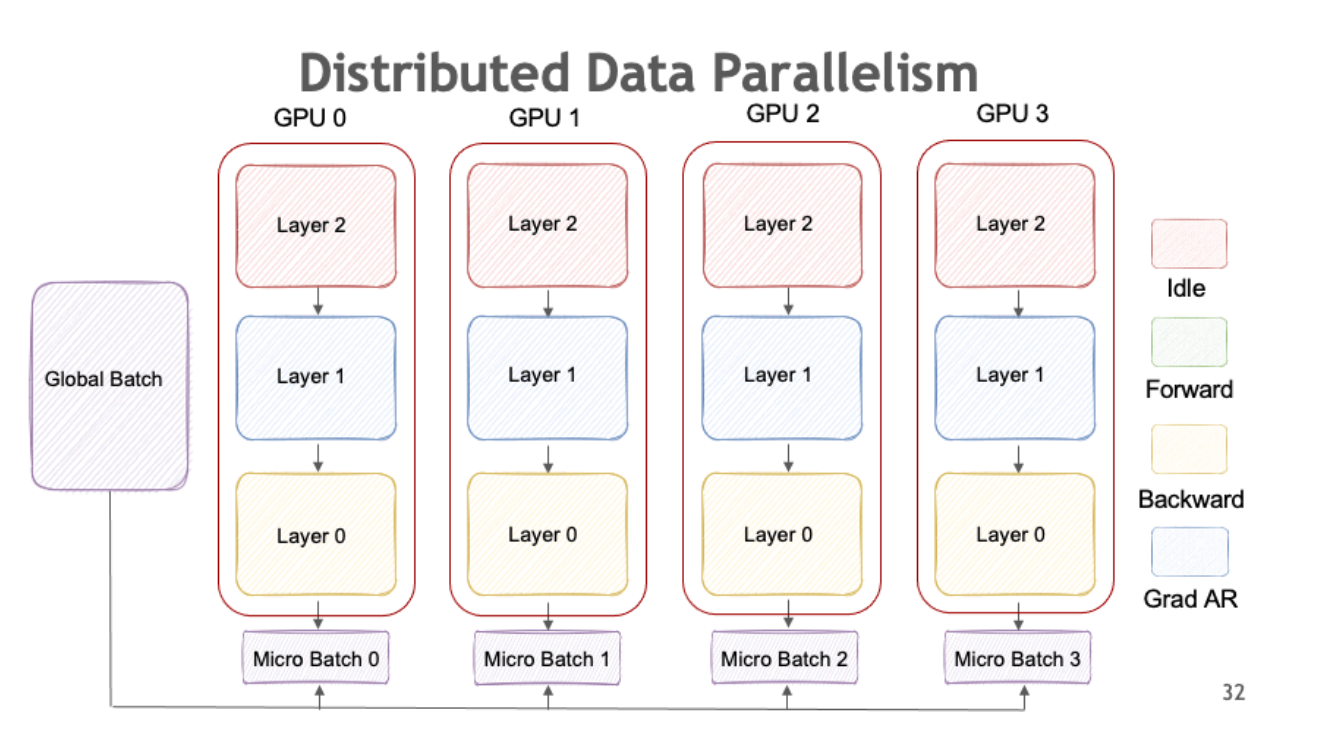
\includegraphics[width = 11cm]{./figure/data_parallel.png} \\ 
	{\footnotesize Source: \href{https://docs.nvidia.com/nemo-framework/user-guide/latest/nemotoolkit/features/parallelisms.html#distributed-data-parallelism}{Nvidia}}
\end{figure}

\vfill

\end{vbframe}

% ------------------------------------------------------------------------------

\begin{vbframe}{Data Parallelism (2)}
\begin{itemize}
    \item \textbf{Data Splitting:}
        \begin{itemize}
            \item The dataset is divided into smaller chunks, and each chunk is assigned to a different processing unit (e.g., GPU or CPU) on different nodes
            \item Each node processes a different subset of the data in parallel, reducing the overall training time    
        \end{itemize}
    \item \textbf{Model Replication:}
        \begin{itemize}
            \item Each processing unit has a replica of the neural network model
            \item These replicas are trained independently on their respective data subsets
        \end{itemize}
    \item \textbf{Gradient Aggregation:}
        \begin{itemize}
            \item After each forward and backward pass, gradients are computed locally on each node 
            \item The gradients are then averaged (or summed) across all nodes to ensure that each model   replica receives the same gradient update     
        \end{itemize}
    \item \textbf{Parameter Synchronization:}
        \begin{itemize}
            \item The model parameters (weights and biases) are updated synchronously across all nodes
            \item This ensures that all model replicas remain consistent with each other after each update step    
        \end{itemize}
\end{itemize}

\end{vbframe}

% ------------------------------------------------------------------------------

\begin{vbframe}{Tensor Parallelism (1) (Animated GIF!)}

\vfill

\begin{figure}
	\centering
	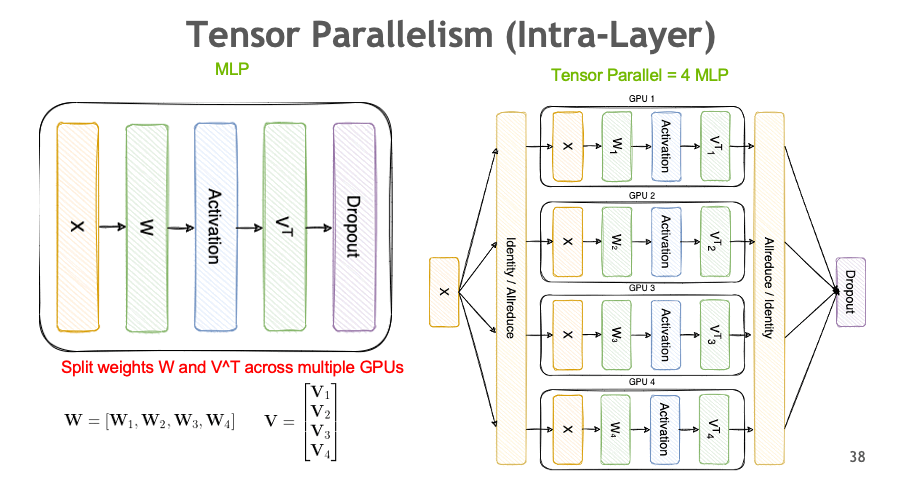
\includegraphics[width = 11cm]{./figure/tensor_parallel.png} \\ 
	{\footnotesize Source: \href{https://docs.nvidia.com/nemo-framework/user-guide/latest/nemotoolkit/features/parallelisms.html#tensor-parallelism}{Nvidia}}
\end{figure}

\vfill

\end{vbframe}

% ------------------------------------------------------------------------------

\begin{vbframe}{Tensor Parallelism (2)}

\begin{itemize}
    \item \textbf{Model Partitioning:}
    \begin{itemize}
        \item The model's layers or tensors are split across multiple devices
        \item Different parts of the model are assigned to different devices, enabling them to work on separate portions of the computations simultaneously
    \end{itemize}
    
    \item \textbf{Forward and Backward Passes:}
    \begin{itemize}
        \item During the forward pass, each device processes its portion of the tensors with intermediate results passed between devices
        \item In the backward pass, gradients are computed in the reverse order, again with necessary data transfers between devices
    \end{itemize}    
    \item \textbf{Parameter Updates:}
    \begin{itemize}
        \item Parameter updates can be performed independently on each device for the parameters they own
        \item After each update step, the devices synchronize to ensure consistency across the distributed model
    \end{itemize}
\end{itemize}
    
\end{vbframe}

% ------------------------------------------------------------------------------


% \begin{vbframe}{Zero Redundancy Optimizer}

% \vfill

% \begin{figure}
% 	\centering
% 	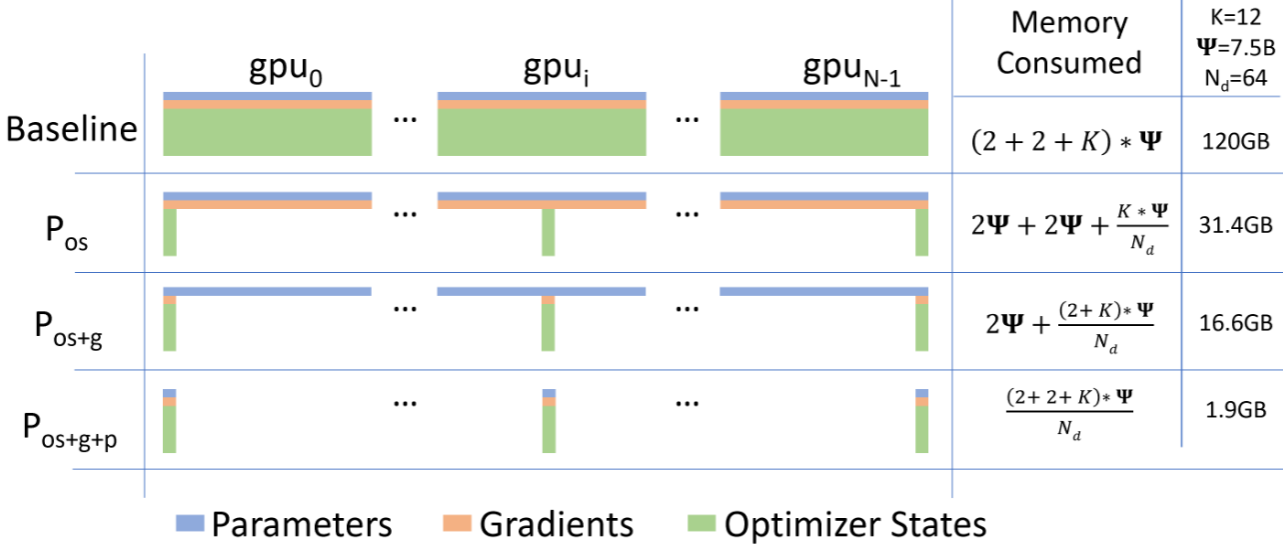
\includegraphics[width = 11cm]{./figure/zero_paralel.png} \\ 
%  \caption{Comparing the per-device memory consumption of model states, with three stages of ZeRO-DP optimizations.}
%   \citebutton{Rajbhandari et al., 2020}{https://arxiv.org/pdf/1910.02054.pdf}
  
% \end{figure}

% \vfill

% \end{vbframe}

% ------------------------------------------------------------------------------

\begin{vbframe}{F\MakeLowercase{lash}A\MakeLowercase{ttention}}

\vfill

Fast and Memory-Efficient Exact Attention with IO-Awareness \newline

\begin{itemize}
	\item Fast
	\begin{itemize}
		\item 15\,\% faster than BERT
		\item 3x faster than GPT-2 
		\item 2.4x faster than Megatron-LM
	\end{itemize}
	\item Memory-efficient
	\begin{itemize}
		\item Reducing from $O(\MakeLowercase{n}^2)$ to $O(\MakeLowercase{n})$ 
	\end{itemize}
	\item Exact
	\begin{itemize}
		\item Same as ``vanilla attention'', not an approximation 
	\end{itemize}
	\item IO aware
	\begin{itemize}
		\item Reducing memory load/store operations
	\end{itemize}
\end{itemize}

\vfill

\end{vbframe}

% ------------------------------------------------------------------------------

\begin{vbframe}{GPU Memory Hierarchy}

\vfill

\begin{figure}
	\centering
	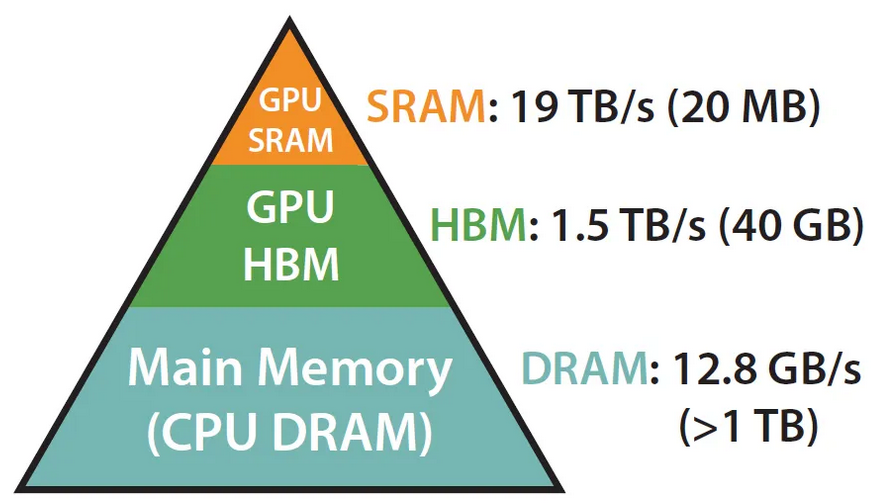
\includegraphics[width = 11cm]{./figure/gpu_mem.png} \\ 
	{\footnotesize Source: \href{https://arxiv.org/abs/2205.14135}{Dao et al. (2022)}}
\end{figure}

\vfill

\end{vbframe}

% ------------------------------------------------------------------------------

\begin{vbframe}{Computing Considerations}

\vfill

\begin{itemize}
	\item GPU compute has been growing faster than memory bandwidth
	\begin{itemize}
		\item GPU has to wait for data
	\end{itemize}
	\item Transformer operations are memory-bound
	\begin{itemize}
		\item Elementwise operations with high memory access
	\end{itemize}
	\item IO aware means reducing memory load/store operations
	\item FlashAttention implements the following:
	\begin{itemize}
		\item Operation fusion to reduce memory access
		\item Tiling or chunking the softmax matrix into blocks
		\item Recomputation for better memory utilization
	\end{itemize}
\end{itemize}

\vfill

\end{vbframe}

% ------------------------------------------------------------------------------

\begin{vbframe}{Operation Fusion}

\vfill

\begin{figure}
	\centering
	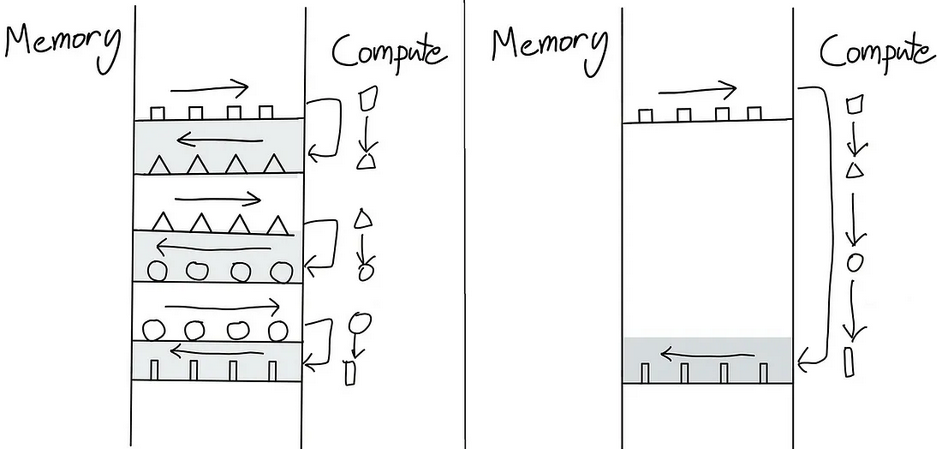
\includegraphics[width = 11cm]{./figure/op_fusion.png} \\ 
	{\footnotesize Source: \href{https://horace.io/brrr_intro.html}{\url{https://horace.io/brrr_intro.html}}}
\end{figure}

\vfill

\end{vbframe}

% ------------------------------------------------------------------------------

% \begin{vbframe}{Operation Fusion (2)}
%     \begin{itemize}
%     \item \textbf{Definition:}
%     \begin{itemize}
%         \item Operation Fusion refers to the technique of combining multiple operations into a single operation.
%         \item This is done to reduce the computational overhead and improve performance.
%     \end{itemize}
    
%     \item \textbf{Purpose:}
%     \begin{itemize}
%         \item The primary goal is to enhance the efficiency of the attention mechanism.
%         \item By fusing operations, it reduces the number of memory accesses and computational steps.
%     \end{itemize}
    
%     \item \textbf{Application in FlashAttention:}
%     \begin{itemize}
%         \item Flash Attention uses operation fusion to optimize the attention computation.
%         \item Key steps in the attention mechanism are fused to streamline the process.
%     \end{itemize}
% \end{itemize}

% \end{vbframe}

% ------------------------------------------------------------------------------

\begin{vbframe}{Limitations and Prospects}

\vfill

\begin{itemize}
	\item FlashAttention requires writing attention to CUDA language
	\begin{itemize}
		\item A new CUDA kernel for each new attention implementation
		\item CUDA is lower-level than PyTorch
		\item Implementation may not be transferable accross GPUs
	\end{itemize}
	\item Towards IO-Aware Deep Learning
	\begin{itemize}
		\item Extending beyonde attention
	\end{itemize}
	\item Multi-GPU IO-Aware Methods
	\begin{itemize}
		\item FlashAttention computation may be parallelizable accross multiple GPUs
	\end{itemize}
\end{itemize}

\vfill

\end{vbframe}

% ------------------------------------------------------------------------------

\endlecture
\end{document}